\subsection{Összefoglaló feladatok}


\newcounter{feladatSzamlalo}

%_
\begin{frame}
  Készítse el a \hiv{\href{https://hu.wikipedia.org/wiki/Cascading_Style_Sheets}{CSS wiki oldala}} által ihletett weblapot!
  \begin{columns}[c]
    \column{0.25\textwidth}
      \begin{exampleblock}{\textattachfile{css.html}{css.html}}
        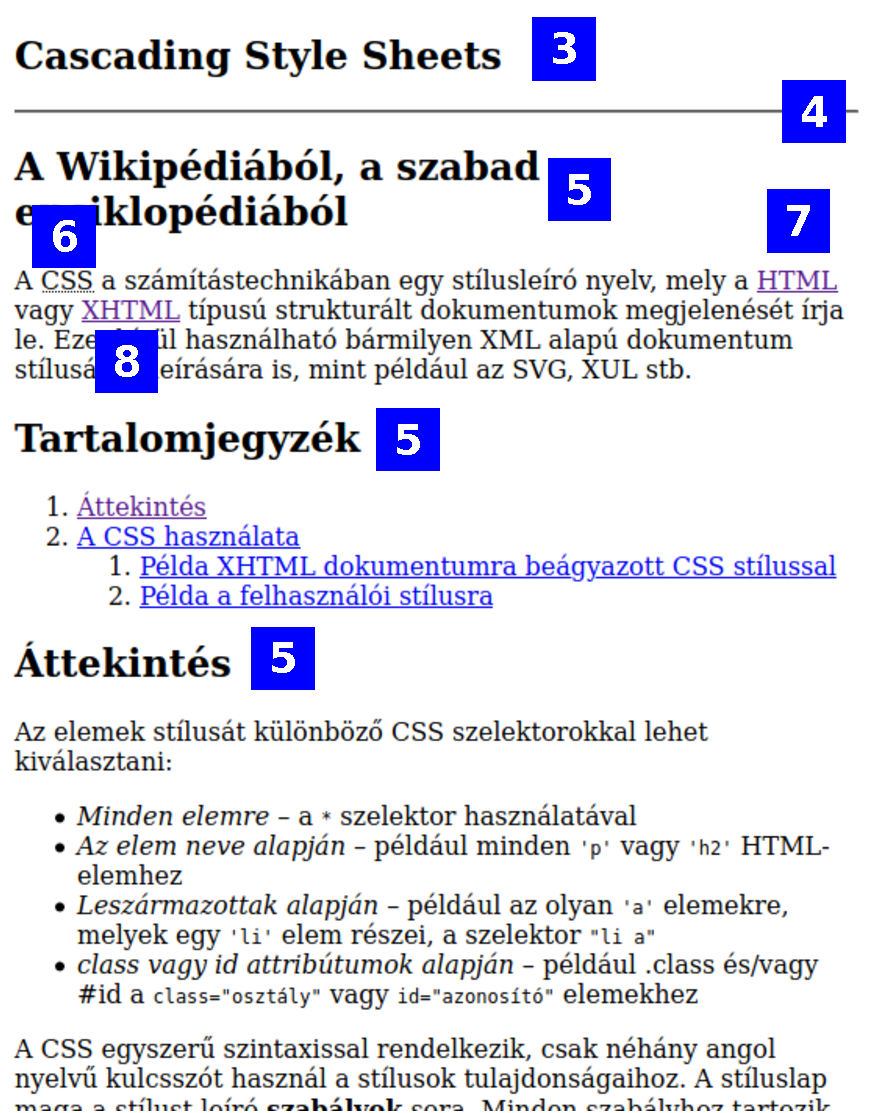
\includegraphics[width=\textwidth]{css1.pdf}
      \end{exampleblock}
    \column{0.75\textwidth}
      \begin{enumerate}
        \scriptsize
        \item Induljon ki a \textattachfile{css.txt}{css.txt} fájlból!
        \item Készítsen ebből magyar nyelvű HTML5 dokumentumot, UTF-8 karakterkódolással!
        \item Az oldal első szintű címsora és a böngészőfülön megjelenő szöveg egyaránt legyen ,,Cascading Style Sheets''!
        \item Ezt válassza el egy vízszintes vonallal...
        \item ...a második szintű címsorként jelölt sortól (,,A Wikipédiából, \dots'')! A ,,Tartalomjegyzék'' és az ,,Áttekintés'' szintén 2. szintű címsorként legyen jelölve!
        \item Az első bekezdés elején álló ,,CSS''-t jelölje meg rövidítésként! Ha valaki fölötte tartja az egeret, jelenjen meg a ,,Cascading Style Sheets, magyarul: lépcsőzetes stíluslapok'' szöveg egy buborékban!
        \item Jelölje meg hivatkozásként a ,,HTML'' szót, ami a megfelelő Wikipédia oldalra mutat!
        \item Járjon el ugyanígy az ,,XHTML''-lel is, de azt új fülön nyissa meg!
        \setcounter{feladatSzamlalo}{\theenumi}
      \end{enumerate}
  \end{columns}
\end{frame}

%_
\begin{frame}
  \begin{columns}[c]
    \column{0.25\textwidth}
      \begin{exampleblock}{\textattachfile{css.html}{css.html}}
        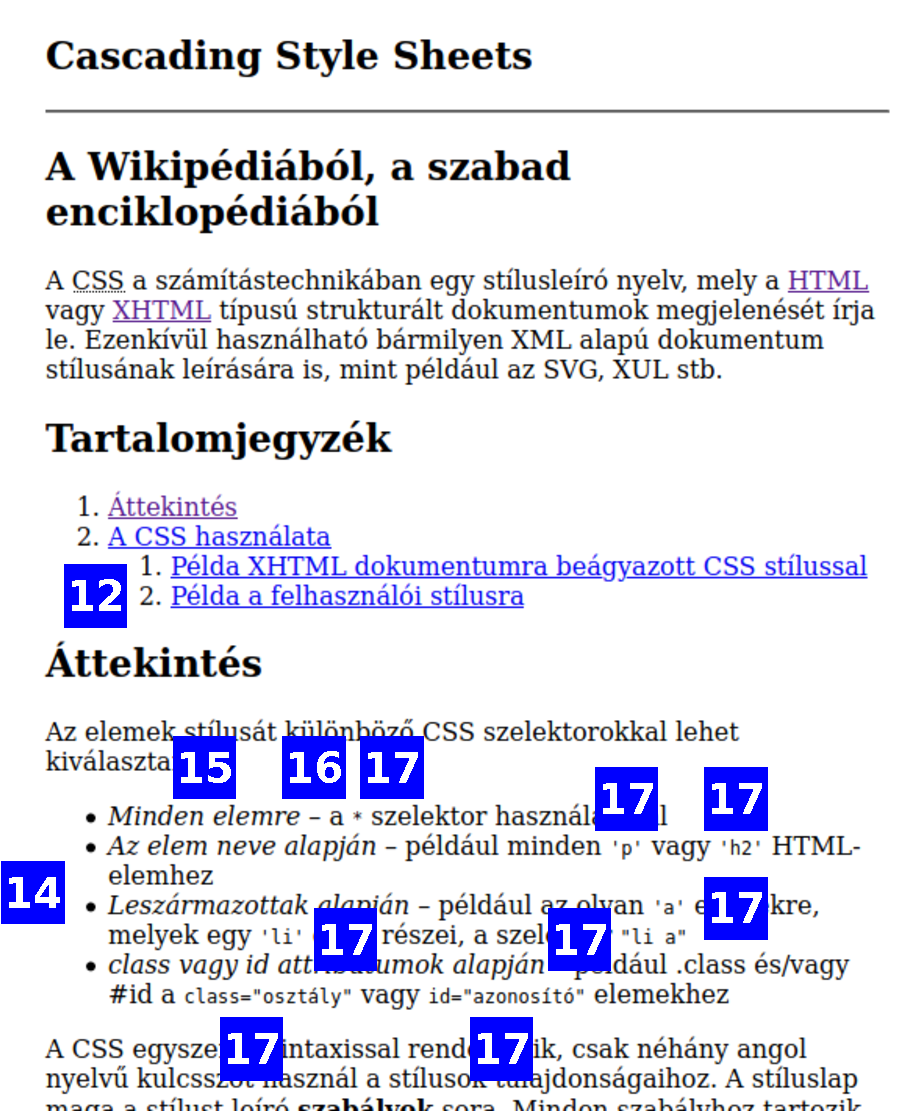
\includegraphics[width=\textwidth]{css2.pdf}
      \end{exampleblock}
    \column{0.75\textwidth}
      \begin{enumerate}
        \footnotesize
        \setcounter{enumi}{\thefeladatSzamlalo}
        \item A dokumentum tartalma alkosson egy cikket!
        \item Minden, ami a tartalomjegyzék felett van, legyen fejlécként jelölve!
        \item Külön szakaszként jelölje a tartalomjegyzéket, és az azt követő fő fejezeteket (,,Áttekintés'', ,,A CSS használata'')!
        \item A tartalomjegyzék pontjait egymásba ágyazott, számozott listák alkossák!
        \item Ezek egyúttal legyenek hivatkozások a dokumentumon belüli fejezetekre!
        \item Az ,,Áttekintés'' fejezetben hozzon létre nem számozott felsorolást!
        \item A kötőjel előtti részt jelölje meg hangsúlyos szövegrészként!
        \item A kötőjeleket cserélje közepes hosszúságú gondolatjelekre!
        \item A felsorolás pontjaiban szereplő *-ot, HTML elemneveket, stb. jelölje meg programkódként!
        \setcounter{feladatSzamlalo}{\theenumi}
      \end{enumerate}
  \end{columns}
\end{frame}

%_
\begin{frame}
  \begin{columns}[c]
    \column{0.25\textwidth}
      \begin{exampleblock}{\textattachfile{css.html}{css.html}}
        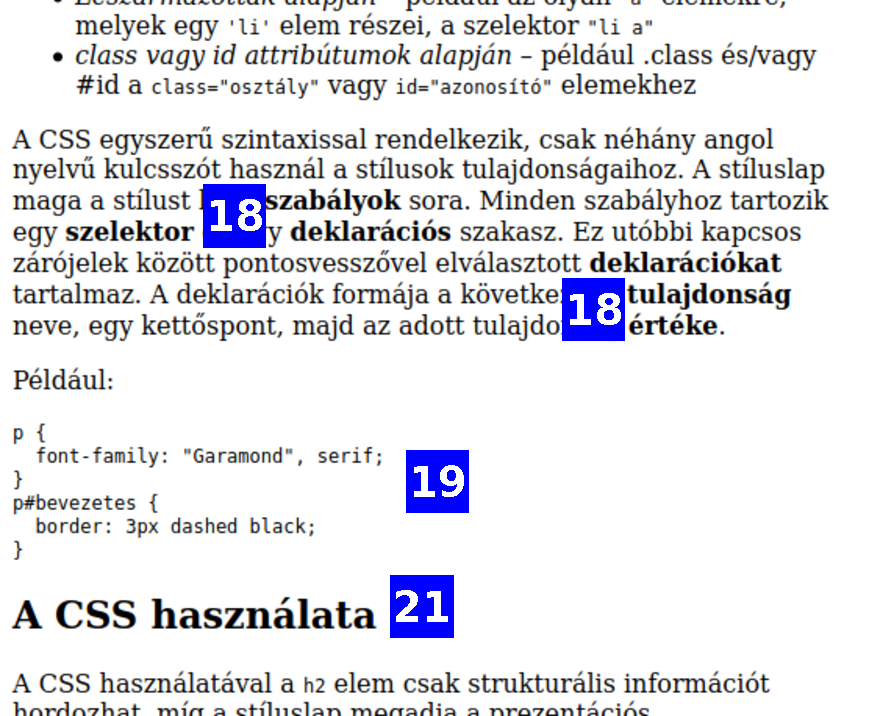
\includegraphics[width=\textwidth]{css3.pdf}
      \end{exampleblock}
    \column{0.75\textwidth}
      \begin{enumerate}
        \setcounter{enumi}{\thefeladatSzamlalo}
        \small
        \item A felsorolást követő szövegben a fontos fogalmakat (szabályok, szelektor, deklarációs, \dots) jelölje meg félkövérrel szedendő szövegként!
        \item A példaként szereplő CSS szöveget jelölje meg előformázott szövegrésznek!
        \item A CSS kód töredékeit ágyazza be olyan, előredefiniált jelentéssel nem bíró soron belüli elembe, melynek \texttt{class} attribútuma utal a kód azon részének szemantikai töltetére! A \texttt{p} elemneveknél az attribútum értéke legyen \texttt{element}, a \texttt{bevezetes}-nél \texttt{id}, a \texttt{font-family} és \texttt{border} tulajdonságnál \texttt{property}, a kettőspont utáni részeknél \texttt{keyword}, kivéve a \texttt{"Garamond"}-ot, amit jelöljön \texttt{string}-nek, a \texttt{3}-at, amit \texttt{quantity}-nak, a \texttt{px}-et pedig \texttt{unit}-nak!
        \item Jelölje meg 2. szintű címsorként ,,A CSS használata'' sort!
        \setcounter{feladatSzamlalo}{\theenumi}
      \end{enumerate}
  \end{columns}
\end{frame}

%_
\begin{frame}
  \begin{columns}[c]
    \column{0.25\textwidth}
      \begin{exampleblock}{\textattachfile{css.html}{css.html}}
        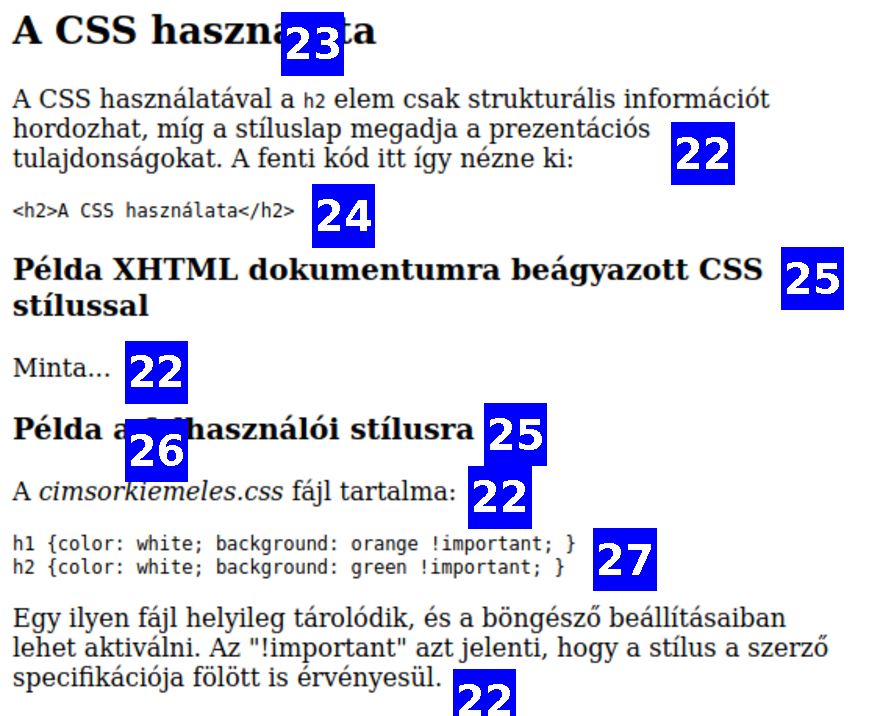
\includegraphics[width=\textwidth]{css4.pdf}
      \end{exampleblock}
    \column{0.75\textwidth}
      \begin{enumerate}
        \setcounter{enumi}{\thefeladatSzamlalo}
        \item Jelölje meg a bekezdéseket!
        \item A fejezet első bekezdésében szereplő \texttt{h2}-t jelölje meg programkódként!
        \item A következő, minta kód legyen előformázott szövegnek jelölve! Figyeljen rá, hogy minden karakter megjelenjen, és ne kezdje értelmezni azokat a böngészőprogram!
        \item Jelölje meg a ,,Példa XHTML dokumentumra\dots'' és ,,Példa a felhasználói\dots'' sorokat 3. szintű címsornak!
        \item Jelölje meg a fájlnevet dőlt betűs szövegként!
        \item A CSS szövegrészt jelölje előformázott szövegként!
        \setcounter{feladatSzamlalo}{\theenumi}
      \end{enumerate}
  \end{columns}
\end{frame}

%_
\begin{frame}
  Készítse el a \textattachfile{szamla.txt}{szamla.txt} szövegének felhasználásával az alábbi számlát!
  \begin{columns}[c]
    \column{0.5\textwidth}
      \begin{itemize}
        \small
        \item A dokumentum legyen UTF-8 kódolású, a böngészőfülön álljon \emph{Számla} felirat!
        \item Kapcsolja össze a HTML fájlt a \textattachfile{szamla.css}{szamla.css} stíluslappal!
        \item Helyezzen el a HTML fejrészében olyan leírást, amely a ,,Számla, táblázatok gyakorlásához'' szöveget tartalmazza!
        \item A számlát egy külső táblázatból, és az annak fejrészébe, törzsébe, lábrészébe beágyazott táblázatokból lehet összeállítani. Ügyeljen az általános és fejléc cellák közötti különbségekre is!
      \end{itemize}
    \column{0.5\textwidth}
      \begin{exampleblock}{\textattachfile{szamla.html}{szamla.html}}
        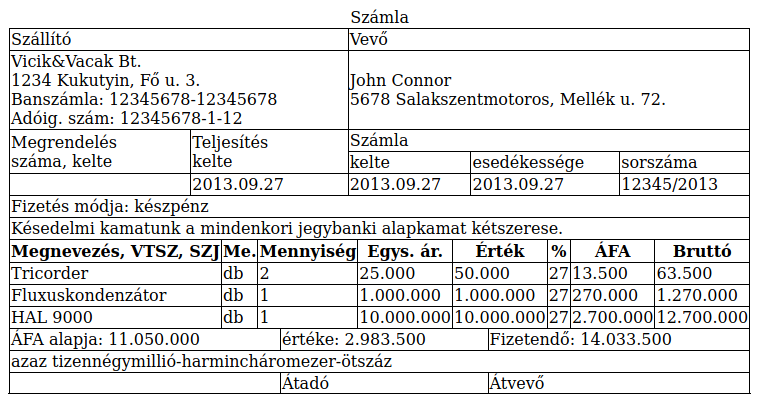
\includegraphics[width=\textwidth]{szamla.png}
      \end{exampleblock}
  \end{columns}
\end{frame}

%_
\begin{frame}
  \begin{columns}[c]
    \column{0.6\textwidth}
      Készítse el az űrlapot!
      \begin{itemize}
        \scriptsize
        \item A dokumentum legyen UTF-8 kódolású, a böngészőfülön álljon \emph{Űrlap} felirat, szövegét jelölje meg magyarként!
        \item Az űrlap tartalmát küldje \texttt{POST} módszerrel a \texttt{http://xenia.sze.hu/\textasciitilde wajzy/feldolgozo.php} címre!
        \item A beviteli mezők előtt álló magyarázó feliratok legyenek a vezérlővel összekapcsolt címkék!
        \item A ,,Név'' és ,,Életkor'' első betűit jelenítse meg félkövér betűkkel!
        \item Ezek a kiemelt betűk legyenek a vezérlő fókuszba kerülésének gyorsbillentyűi! (Többnyire \texttt{Alt+Shift+}\emph{gyorsbillentyű})
        \item Névként legfeljebb 64 karaktert lehessen bevinni, és jelenítsen meg helykitöltő szöveget arra az időre, amíg a felhasználó nem ad meg adatot!
        \item Az életkornál csak 0 és 120 közé eső számokat lehessen megadni, és kötelező kitölteni.
      \end{itemize}
    \column{0.35\textwidth}
      \begin{exampleblock}{\textattachfile{urlap.html}{urlap.html}}
        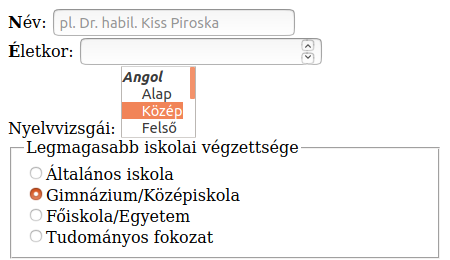
\includegraphics[width=\textwidth]{urlap-1.png}
      \end{exampleblock}
  \end{columns}
\end{frame}

%_
\begin{frame}
  \begin{columns}[c]
    \column{0.6\textwidth}
      \begin{itemize}
        \small
        \item Nyelvvizsgákból lehessen egyszerre többet is kijelölni! Angol és német nyelvből (ezek legyenek a csoportok címkéi) is lehet alap-, közép- és felsőfokú vizsgát megadni. Az angol középfok már az oldal betöltésekor legyen alapértelmezetten kiválasztva!
        \item Vegye körbe a rádiógombokat egy dobozzal, melyben a ,,Legmagasabb iskolai végzettsége'' felirat olvasható!
        \item A rádiógombok egy csoportot alkotnak, az oldal betöltésekor a ,,Gimnázium/Középiskola'' legyen kiválasztva!
      \end{itemize}
    \column{0.35\textwidth}
      \begin{exampleblock}{\textattachfile{urlap.html}{urlap.html}}
        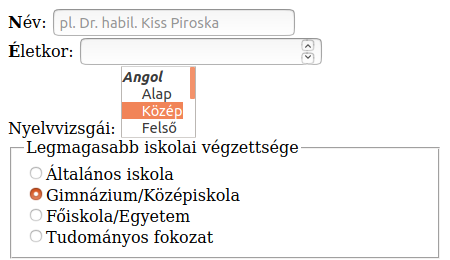
\includegraphics[width=\textwidth]{urlap-1.png}
      \end{exampleblock}
  \end{columns}
\end{frame}

%_
\begin{frame}
  \begin{columns}[c]
    \column{0.6\textwidth}
      \begin{itemize}
        \item Készítse el a hobbyk csoportját a megfelelő felirattal!
        \item Álljanak ezek jelölőnégyzetekből!
        \item A bemutatkozás szövegbeviteli mezője 40 oszlop széles, 10 sor magas legyen! Legyen benne már egy sor szöveg!
        \item Az önéletrajznál lehessen több fájlt is feltölteni egyszerre!
        \item Helyezzen el az űrlap küldésére és alaphelyzetbe állítására szolgáló gombokat!
      \end{itemize}
    \column{0.35\textwidth}
      \begin{exampleblock}{\textattachfile{urlap.html}{urlap.html}}
        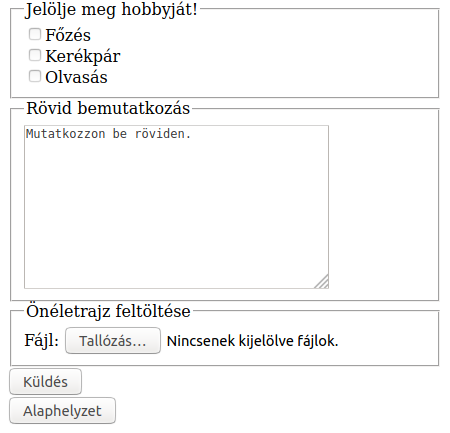
\includegraphics[width=\textwidth]{urlap-2.png}
      \end{exampleblock}
  \end{columns}
\end{frame}

%_
\begin{frame}
  Az eredmény a megadott adatoktól, a vezérlők nevétől függően az alábbihoz hasonló lehet:
  \begin{center}
    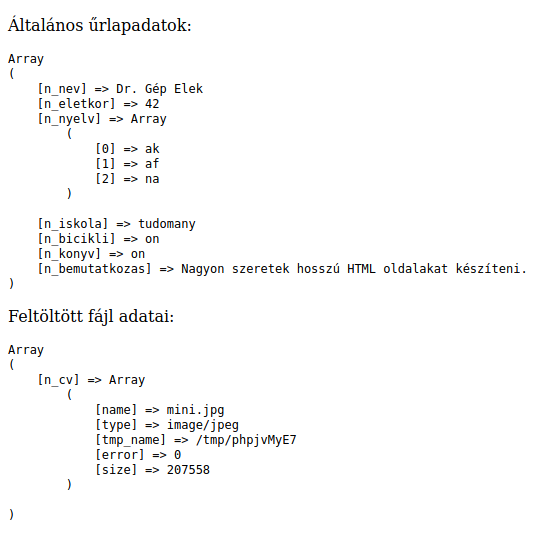
\includegraphics[width=.4\textwidth]{urlap-3.png}
  \end{center}
\end{frame}
